\providecommand{\main}{..}

\documentclass[/home/francois/latex/report/main.tex]{subfiles}

\begin{document}

\chapter{Background}
\label{chapter:background}

A lot of effort have been put into estimating the dynamic parameters of each rigid body link of robotic manipulators during the late century spent. An et al. \cite{An1985} have developped a method to estimate the mass, the location of the center of mass and the moment of inertia of every link of a robotic arm. The method uses the joint torques and the calculation of the kinematics of the manipulator while moving. This work provide a sound method to derive the dynamic equations (see Section \ref{subsection:background_newton_equation} and \ref{subsection:method_newton_equation}).

\textit{TODO}

{\it
The estimation of the inertial parameters of an object attached to a manipulator was being addressed by researchers only within the last two decades.
}

\section{Hardware setup}



\section{Description of the Problem}
\label{section:description}

\textit{TODO}

\begin{figure}[H]
  \centering
  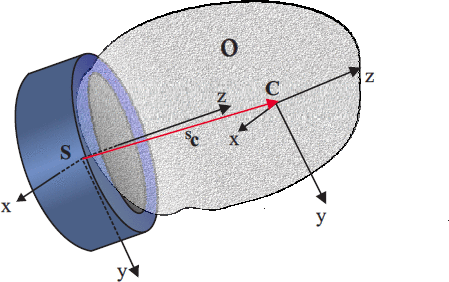
\includegraphics[scale=0.4]{\main/figures/scheme.png}
  \caption{2-bodies with 2-dimensions assumptions system.}
  \label{fig:background:payload_sensor}
\end{figure}

\begin{itemize}
 \item \ac{FT} sensor measuring: force $f$ and torque $\tau$,
 \item payload attached to the \ac{FT} sensor: mass $m$, center of mass $c$, moment of inertia $I$, linear acceleration $a$, angular acceleration $\alpha$, angular velocity $\omega$,
\end{itemize}

\section{Dynamic Model}

\subsection{Formulation of the \textsc{Newton-Euler} equations}
\label{subsection:background_newton_equation}

\textit{TODO}

Dynamic model of the load rigidly attached to the manipulator

The motion of the body due to external forces is described by the two equations \cite{Kubus2007, Kubus2008}:

\begin{equation}
 \label{dim_1}
 \left \{
 \begin{array}{l l}
  f =    & m (a - g) + \dot{\theta} \times (\dot{\theta} \times m c) + \ddot{\theta} \times m c \\
  \tau = & m c \times (a - g)
  + I_{S} \ast \ddot{\theta} + \dot{\theta} \times (I_{S} \ast \dot{\theta})
 \end{array}
 \right.
\end{equation}

also in matrix form:

\begin{equation}
 \begin{pmatrix}
  f    \\
  \tau
 \end{pmatrix}
 = A(a, \alpha, \omega, g) \varphi
\end{equation}

with $\varphi = (m, m c_x, m c_y, m c_z, I_{xx}, I_{xy}, I_{xz}, I_{yy}, I_{yz}, I_{zz}) {}^T$

\subsection{Sensor offset}

\textit{TODO}

{\it
Strategies to manage the (unknown) sensor offset \cite{Kubus2007, Kubus2008}.
}

\section{Estimation Approaches}

\subsection{Least-Squares method}

\textit{TODO}

{\it
Brief presentation of the method in order to highlight the limit of the least-squares method.
}

\subsection{Recursive Total Least-Squares technique}

\textit{TODO}

{\it
Recursive Total Least-Squares considers error $E$ in the data matrix and error $e$ in the \ac{FT} vector \cite{Kubus2008}
.

\begin{equation}
 \begin{pmatrix}
  f    \\
  \tau
 \end{pmatrix} + e
 = (A + E) \varphi
\end{equation}
}

\end{document}
